%\documentclass{beamer}
\documentclass[xcolor=dvipsnames]{beamer}
\usepackage[latin1]{inputenc}
\usepackage{hyperref}
\usecolortheme[named=Violet]{structure}
\usetheme{Warsaw}
\usepackage{listings}
\usepackage{color}
\usepackage{framed}

\definecolor{dkgreen}{rgb}{0,0.6,0}
\definecolor{gray}{rgb}{0.5,0.5,0.5}
\definecolor{mauve}{rgb}{0.58,0,0.82}

% "define" julia
\lstdefinelanguage{julia}{morekeywords={function,if,else,while,for,:,end}, sensitive=true, morecomment=[l]{\#}, morecomment=[s]{/*}{*/}, morestring=[b]"}

% Default settings for code listings
\lstset{frame=tb,
   language=julia,
   aboveskip=3mm,
   belowskip=3mm,
   showstringspaces=false,
   columns=flexible,
   basicstyle={\small\ttfamily},
   numbers=none,
   frame=none,
   numberstyle=\tiny\color{gray},
   keywordstyle=\color{blue},
   commentstyle=\color{dkgreen},
   stringstyle=\color{mauve},
   breaklines=true,
   breakatwhitespace=true
   tabsize=3
}

\title[Scientific Computing]{Elements of Scientific Computing with Julia}
\begin{document}

\begin{frame}
\titlepage
\end{frame}

\AtBeginSubsection[]
{
  \begin{frame}<beamer>
    \frametitle{Today's Class}
    \tableofcontents[currentsection,currentsubsection]
  \end{frame}
}
\section{Linear Regression with One Variable}
\begin{frame}
{\bf Fitting a Line to Data}

{\it\huge L}inear regression is a \emph{statistical learning} approach for quantitatively predicting an outcome {\bf y} on the basis of predictor variables {\bf x}$_i$, such that the relationship between the outcome and the variables is linear. Mathematically we write: \pause
\[
\textnormal{{\bf y}} \approx  \theta_0 +
\theta_1 \textnormal{{\bf x}}_1 +
\theta_2 \textnormal{{\bf x}}_2 + ... +
\theta_n \textnormal{{\bf x}}_n
\]
\pause
that is {\bf y} can be approximated by a linear combination of $n$ predictor variables.\\
\end{frame}

\begin{frame}
{\bf Fitting a Line to Data}
In this lecture we will focus our attention on \emph{single} variable regression and leave the multivariable case for the next lecture. In the single variable case we have that the outcome {\bf y} can be approximated by a linear relationship involving only one input variable {\bf x}, or mathematically: \pause
\[
\textnormal{{\bf y}} \approx  \theta_0 +
\theta_1 \textnormal{{\bf x}}
\]
\end{frame}

\begin{frame}
{\bf Supervised Learning}
There are different contexts in which we may discuss the topic of linear regression. In this lecture, we will study it in the light of machine learning and thus use vocabulary pertinent to this field. \vfill \pause In machine learning there are two main sorts of problems:\pause
\begin{itemize}
\item \emph{supervised learning} and 
\item \emph{unsupervised learning}
\end{itemize}
\vfill \pause In this course we will only address supervised learning problems. \\
\end{frame}

\begin{frame}
{\bf Supervised Learning}
In supervised learning, we wish to infer a function that classifies or fits future data, based on a \emph{training data set:} \vfill\pause
\emph{data that we already have collected and know the ``right'' output for each input}
\vfill\pause 
Let us motivate our discussion with an example. Consider the following training data set on the next slide, where we have on the left column the number of years for which a person went to school and on the right column the income they now make, in thousands of dollars per year.\\
\end{frame}

\begin{frame}[fragile]
{\bf Example: Education v. Income}
\begin{verbatim}
"Education"    "Income"
 10.0           26.6588   
 10.4013        27.3064   
 10.8428        22.1324   
 11.2441        21.1698   
 11.6455        15.1926   
 12.087         26.399    
 12.4883        17.4353   
 12.8896        25.5079   
 13.291         36.8846   
 13.7324        39.6661   
 14.1338        34.3963   
 14.5351        41.498    
 ...                
\end{verbatim}  
\end{frame}

\begin{frame}
{\bf Example: Education v. Income}
\begin{itemize}
\item ``$x$'' or input is the education level of an individual
\item ``$y$'' or output is the income level of the same individual
\end{itemize}
\pause
Since we have many inputs for different observations (say $m$ of them), then we put them all in a $m \times 1$ vector {\bf x}.\vfill \pause 
Similarly, {\bf y} is a $m \times 1$ vector of outputs. \vfill\pause
In linear regression, we wish to infer the function of the line that best fits data in a certain input-output relationship, that is, we wish to come up with a linear function \pause
\[
\textnormal{{\bf h$_{\theta}$(x)}} =  \theta_0 +
\theta_1 \textnormal{{\bf x}}
\]
\pause that best approximates our output vector {\bf y}.
\end{frame}

\begin{frame}
{\bf Example: Education v. Income}
In the formula above we have that $\theta_i$'s are the \emph{parameters} or the \emph{weights} of the linear map from {\bf x} to {\bf y}. \vfill\pause So we want to find the parameters (in this case they are the slope and $y$-intercept of our line) that give us a line of best fit as in the picture below:
\pause
\begin{center}
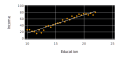
\includegraphics[scale=.75]{myplot.png}
\end{center}
\end{frame}

\begin{frame}
{\bf How to Choose the $\theta$'s?}
So how do we choose the parameters $\theta_i$? \vfill\pause 
In this lecture we will do that via the \emph{Gradient Descent Method}.
\vfill\pause  
In the next lecture we will generalize linear regression and gradient descent for multiple variables (that is, multiple input vectors {\bf x}$_i$), and also learn the \emph{Normal Method} for solving for the parameters $\theta_i$. 
\end{frame}

\begin{frame}
{\bf How to Choose the $\theta$'s?}
But before we get into all that, let us get a better intuition for these parameters, simply by experimenting with a few different combinations of $\theta_0$ and $\theta_1$:\vfill \pause
\begin{minipage}{1.2in}
{\small $h(x) = \theta_0 + \theta_1 x$, \\
$\theta_0 = 1.5, \theta_1 = 0$:\\}
\pause
\includegraphics[width=1in]{plot1.png}\\
\end{minipage}
\pause
\begin{minipage}{1.2in}
{\small $h(x) = \theta_0 + \theta_1 x$, \\
$\theta_0 = 0, \theta_1 = 0.5$:\\}
\pause
\includegraphics[width=1in]{plot2.png}\\
\end{minipage}
\pause
\begin{minipage}{1.2in}
{\small $h(x) = \theta_0 + \theta_1 x$, \\
$\theta_0 = 1, \theta_1 = 0.5$:\\}
\pause
\includegraphics[width=1in]{plot3.png}\\
\end{minipage}
\end{frame}

\begin{frame}
{\bf How to Choose the $\theta$'s?}
Note how changing the parameters $\theta_i$ changes the slope and position of our line in the plane. \vfill\pause As an exercise, I encourage you to read different datasets in Julia (with one input variable, where the output is quantitative), scatter plot the data and play around with manually picking the slope and intercept parameters for the line that best fits the data visually.\\
\end{frame}

\begin{frame}
{\bf The Cost Function}
In order for us to be able to apply the gradient descent algorithm for solving our liner regression problem, we will need a function to minimize (as we will see later gradient descent is an algorithm for finding the input that minimizes the output value of a function). \vfill\pause This function is called the \emph{cost function} and it is defined as follows:\pause
\[
C(\theta_0, \theta_1) = \frac{1}{2m}\sum\limits_{i=1}^m(h_{\theta} (x^{(i)}) - y^{(i)})^2
\]
\end{frame}

\begin{frame}
{\bf The Cost Function}
This function outputs the sum of the squared errors between the predicted outputs and the actual outputs, given inputs $\theta_0$ and $\theta_1$. \vfill\pause
Thus, minimizing this function means getting the $\theta_0$ and $\theta_1$ that causes $C$ to be smallest. \vfill\pause
It seems intuitive to minimize the magnitude of the errors, but you may be wondering why minimize the squared errors versus just the absolute value of the errors. \vfill\pause
For our purposes, the explanation is simple - minimization means taking derivatives, and therefore the cost function must be continuous and differentiable.
\end{frame}

\begin{frame}
{\bf The Cost Function}
Note that the cost function is a \emph{multivariate quadratic function}.\vfill\pause
If $C$ were a quadratic function of one variable, then in a two dimensional space its graph would look like a concave-up parabola. Such a parabola would have a global minimum at the vertex. \vfill\pause
Analogously, in our case $C$'s graph lives in a three dimensional space and it is a ``bowl-up'' shaped surface, with a global minimum at the base of the bowl.\\
\end{frame}

\begin{frame}
{\bf The Cost Function}
\begin{tabular}{c c}
{\bf The surface plot: } & {\bf The contour plot: }\\
\includegraphics[scale=.33]{cost.png} & \includegraphics[scale=.25]{costContour.png}\\
\end{tabular}
\end{frame}

\section{Gradient Descent}
\begin{frame}
{\bf Gradient Descent}

{\it\huge I}n this section we will explore the gradient descent algorithm for optimizing the cost function defined earlier. \vfill\pause 
The gradient descent algorithm is a type of search algorithm, that is we start with an initial guess and then we update our guess iteratively by some rule. \vfill\pause 
The rule for gradient descent is that from our previous guess we should step down (with some step size) toward the direction of steepest descent.\vfill\pause 
If we iterate this rule in a ``bowl-up'' shaped surface with a not-to-large step size, we shall converge to a minimum.
\end{frame}

\begin{frame}
{\bf The Gradient Descent Algorithm}
\begin{framed}
{\bf Gradient Descent Algorithm for Bivariate Functions}\\

\noindent repeat until convergence \{\\
\indent for $j = 0$ and $j = 1$, simultaneously update:
\[
\theta_j := \theta_j - \alpha \frac{\partial}{\partial \theta_j} C(\theta_0,\theta_1)
\]
\}

\end{framed}
\end{frame}

\begin{frame}
{\bf The Gradient Descent Algorithm}
So we take a guess on each $\theta$, then update each $\theta$ \emph{simultaneously} by taking a step of size $\alpha$ in the respective direction of steepest descent as dictated by the partial derivative of the cost function with respect to the $\theta$ that is being updated. \vfill\pause
The intuition here is that the slope of the tangent line to our current point is the steepest slope we can get on a line that would still include the point.\\
\end{frame}

\begin{frame}
{\bf Choosing $\alpha$}
In machine learning, we call the $\alpha$ parameter ``the learning rate''. \\
 
Note: \pause
\begin{itemize}
\item if $\alpha$ is too large our algorithm may diverge, as our steps will be so large as to ``climb the walls'' of our surface \pause
\item if $\alpha$ is too small, our algorithm may take a long time to converge
\end{itemize}
\pause
Tweaking $\alpha$ can be seen as more of an art than a science and it will depend on your particular problem. \vfill\pause
The best way to check that you are picking a good $\alpha$ is to graph (or otherwise output) your \emph{cost} at each iteration and verify that it is indeed decreasing and the rate of decrease is not too slow.\\
\end{frame}

\begin{frame}
{\bf Let me take that derivative for you...}
Using basic Calculus you can easily verify that:
\begin{framed}
\[
j = 0 \Rightarrow \frac{\partial}{\partial \theta_0}C(\theta_0,\theta_1) = \frac{1}{m}\sum\limits_{i=1}^m(h_{\theta}(x^{(i)})-y^{(i)})
\]

\[
j = 1 \Rightarrow \frac{\partial}{\partial \theta_1}C(\theta_0,\theta_1) = \frac{1}{m}\sum\limits_{i=1}^m(h_{\theta}(x^{(i)})-y^{(i)})\cdot x^{(i)}
\]
\end{framed}
\end{frame}

\begin{frame}
{\bf Back to our Example}
So now we have a powerful tool for determining the $\theta$ parameters in your linear regression model. \vfill\pause
Let's go over the accompanying IJulia notebook for this lecture which illustrates linear regression applied to the education versus income data.
\end{frame}


\section{Homework 6}
\begin{frame}
{\bf Homework 6}
The Advertising data set (found in ``Advertising.csv'' on Canvas or GitHub) has data pertaining to the sales in thousands of units versus the advertising budget in thousands of dollars of different advertising media such as TV, radio and newspaper.\\ \pause
\begin{enumerate}
\item Using linear regression with least squares and gradient descent, as outlined in lecture 6,  determine the line that best fits the relationship between sales and advertising budget for each medium. \pause
\item Plot your solution line against the data for each feature considered (that is, sales versus TV budget, radio budget and newspaper budget).
\end{enumerate}
\end{frame}

\begin{frame}
{\bf Homework 6}

\begin{enumerate}
\setcounter{enumi}{2}
\item Plot the surface of your cost function for each feature considered.\pause
\item Compare your results. Is there a medium for advertising that you would claim to be best above all others? Which one and why? Write a short report of your findings using \LaTeX. Make sure to include your formulas and figures obtained in the process of solving this problem.\pause
\end{enumerate}

{\it Commit and push your .ipynb, .tex, and .pdf files for this homework into your GitHub private repository by 5/19 at 11:59 PM.}
\end{frame}

\end{document}